
\section{Resultados}


\paragraph{Análisis de la Red} \mbox{}\\

En el marco de este estudio, se obtuvieron inicialmente 48 genes asociados con el fenotipo mitocondrial desde la base de datos Human Phenotype Ontology (HPO). Estos genes se relacionaron con funciones celulares esenciales en la mitocondria, como la cadena respiratoria, la biogénesis mitocondrial y la regulación del metabolismo energético. Los genes fueron seleccionados con el objetivo de explorar su posible interrelación dentro de una red de interacciones de proteínas, utilizando la base de datos STRING.

Al realizar el análisis de interacciones utilizando los identificadores de estos 48 genes, se observó que solo 38 genes interaccionaron entre sí dentro de la red generada. Este hallazgo sugirió que, aunque todos los genes descargados estaban asociados con el fenotipo mitocondrial, no todos ellos presentaron interacciones directas en el contexto de las proteínas mitocondriales. En particular, algunos genes no mostraron evidencia de interacción directa con otros genes seleccionados, lo que podría haber indicado que sus roles en la biología mitocondrial no dependían de interacciones proteicas directas o que interactuaban a través de mecanismos más complejos no reflejados en esta red.

\begin{figure}
	\centering
	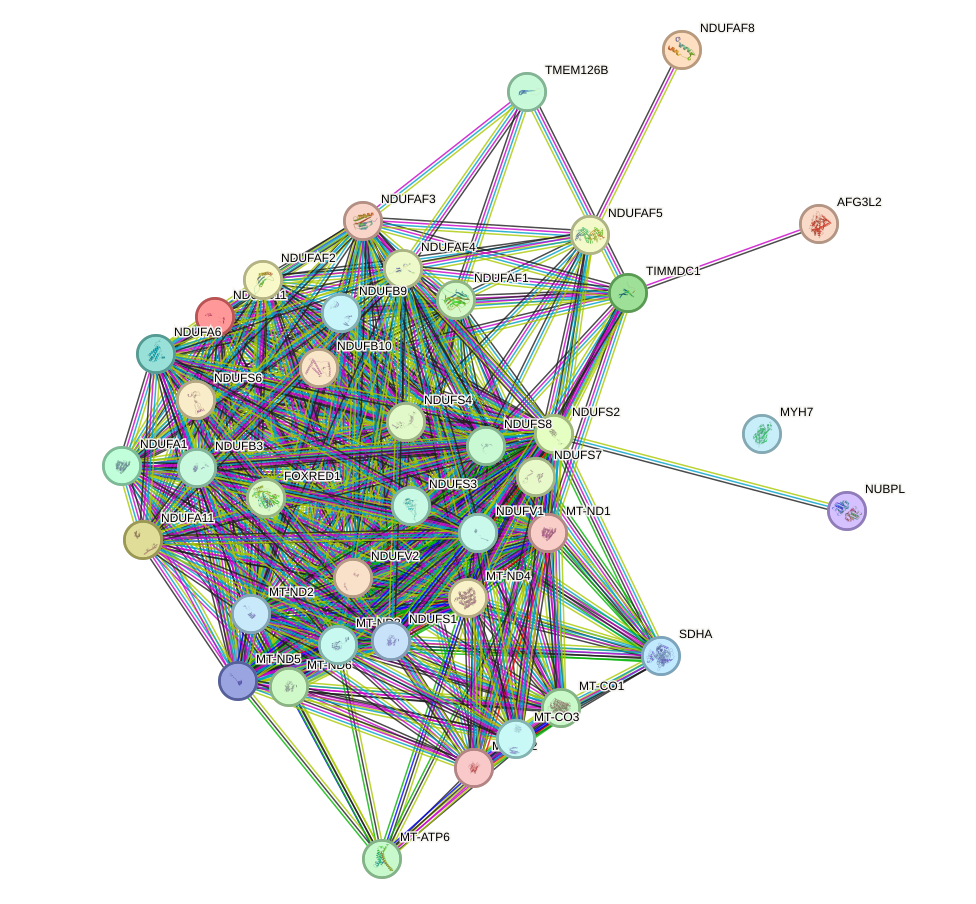
\includegraphics[width=0.8\textwidth]{figures/string_graph.png}
	\caption{Red inicial de nodos}
	\label{fig:imagen1}
\end{figure}

Como puede observarse en la Figura~\ref{fig:imagen1}, uno de los genes más relevantes en este análisis fue MYH7, que estaba relacionado con la miocardiopatía y era conocido por su papel en la función mitocondrial. Sin embargo, MYH7 no presentó interacciones con otros genes mitocondriales en esta red, lo que sugirió que su influencia en el fenotipo mitocondrial podría haber estado mediada por mecanismos independientes, tal vez a través de la regulación de procesos mitocondriales o por interacciones con otras proteínas no incluidas en la red de interacciones analizada.

\paragraph{Clustering} \mbox{}\\

Para profundizar en el análisis de la red obtenida, se han aplicado diferentes algoritmos de clustering con el objetivo de identificar comunidades o grupos de proteínas que interactúen más estrechamente entre sí. Los algoritmos utilizados fueron: Fast Greedy, Edge Betweenness, Walktrap, Infomap y Label Propagation, y se evaluaron mediante la métrica de modularidad, que mide la calidad de las particiones realizadas.
\vspace{1em}

\begin{tabular}{|l|c|r|}
	\hline
	\textbf{Algoritmo} & \textbf{Modularidad} & \textbf{Número de Clusters} \\
	\hline
	Fast Greedy & 0.06917908 & 3 \\
	\hline
	Walktrap clustering & 0.02946764 & 9 \\
	\hline
	Edge Betweenness clustering & 0.01066141 & 1 \\
	\hline
	Infomap clustering & \(2.220446 \times 10^{-16}\) & 1 \\
	\hline
	Label\_Propagation clustering & \(2.220446 \times 10^{-16}\) & 1 \\
	\hline
\end{tabular}


\vspace{1em}
	

Entre los algoritmos evaluados, se observó que Fast Greedy destacó como el algoritmo más efectivo, lo que indicó que logró separar de forma significativa las diferentes comunidades.

El algoritmo identificó tres clúster principales:

En el primer clúster se encontraron nodos como NDUFS7, NDUFAF1, NDUFB10, NDUFS6, NDUFV2. Este clúster reunió muchas proteínas de la familia NDUF, fundamentales para la producción de energía en la célula. Entre estos elementos se observó una alta conectividad.

El segundo clúster contuvo como nodos más destacados MT-CO1, MT-ATP6, MT-ND6, MT-ND5. Este grupo pareció estar más enfocado en la respiración celular y la fosforilación oxidativa.

El tercer clúster estuvo representado por elementos menos conectados, como por ejemplo: NDUFS2, TIMMDC1, NUBPL. Este clúster podría haber indicado que se estaban enfocando en procesos relacionados con la cadena de transporte de electrones. Para un mejor entendimiento, véase la Figura~\ref{fig:imagen2}.

\begin{figure}
	\centering
	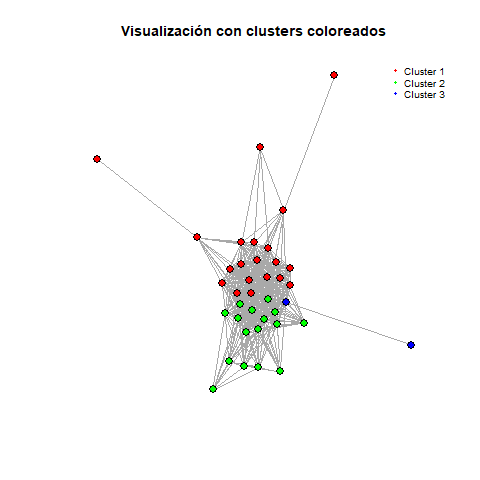
\includegraphics[width=0.8\textwidth]{figures/colored_Fast_Greedy.png}
	\caption{Clustering con algoritmo Fast Greedy}
	\label{fig:imagen2}
\end{figure}

El dendrograma generado mediante clustering jerárquico aportó una perspectiva adicional sobre cómo se relacionaban los genes seleccionados. Esta herramienta organizó los genes en una estructura jerárquica basada en sus similitudes funcionales, permitiendo observar con mayor claridad la proximidad o separación entre ellos dentro de la red de interacciones.

\paragraph{Agrupación de genes} \mbox{}\\

En las ramas inferiores del dendrograma, destacaron genes como \textbf{NDUFS7}, \textbf{NDUFS3} y \textbf{NDUFS6}, los cuales presentaban una alta conectividad en la red de interacciones y se agrupaban estrechamente. Esto reforzó los hallazgos de clustering realizados previamente, donde estos genes se identificaron como parte de comunidades definidas por algoritmos como Fast Greedy. Su proximidad sugirió roles interrelacionados en la producción de energía celular.

\paragraph{Separación de grupos} \mbox{}\\

A medida que se ascendía en la jerarquía, genes como \textbf{NDUFB10} y \textbf{MT-CO1} comenzaban a divergir, formando grupos más distantes. Este patrón era consistente con los resultados del algoritmo Walktrap, donde dichos genes pertenecían a clusters separados, lo que indicaba funciones menos directamente conectadas dentro de la red.

\paragraph{Genes periféricos} \mbox{}\\

En las ramas más alejadas del dendrograma se encontraban genes como \textbf{NUBPL} y \textbf{TIMMDC1}, los cuales presentaban menor conectividad con los clusters principales. Sin embargo, estos genes podrían desempeñar roles complementarios, interactuando de manera más indirecta con genes centrales como \textbf{MT-ATP6}.

\paragraph{Relación entre clusters} \mbox{}\\

La estructura jerárquica observada en el dendrograma confirmó la organización de los clusters identificados previamente. Los genes del primer y segundo cluster mostraron una conexión más estrecha, con roles críticos en la cadena respiratoria y la fosforilación oxidativa. Por otro lado, los genes del tercer cluster aparecieron más tempranamente segregados, sugiriendo funciones complementarias o especializadas dentro del contexto mitocondrial.

\paragraph{}

Tras haber observado la separación en comunidades mediante el uso de diferentes algoritmos de clustering, se procedió a realizar un análisis funcional detallado para cada uno de los grupos identificados. Este análisis tuvo como objetivo explorar las funciones biológicas principales asociadas a los genes de cada comunidad, así como su posible implicación en procesos mitocondriales clave. Adicionalmente, se analizaron los nodos principales (\textbf{top nodes}) de la red, definidos como aquellos genes con mayor conectividad y centralidad, que podrían desempeñar roles esenciales dentro de la red biológica.

\paragraph{Análisis funcional del primer clúster} \mbox{}\\

El primer clúster, que agrupa principalmente proteínas de la familia NDUF (e.g., NDUFS7, NDUFAF1, NDUFB10), mostró un enriquecimiento significativo en procesos relacionados con la organización mitocondrial y el ensamblaje del complejo I de la cadena respiratoria. Entre los términos más destacados se encuentran "NADH dehydrogenase complex assembly" y "mitochondrial respiratory chain complex assembly". Estos resultados refuerzan el papel fundamental de este grupo en la producción de energía celular mediante la fosforilación oxidativa.

El alto \textbf{GeneRatio} (\(\geq 0.6\)) y los valores ajustados de significancia extremadamente bajos (\( 5.6 \times 10^{-40} \)) sugieren que la mayoría de los genes de este clúster están funcionalmente relacionados. Esto subraya la importancia de estos genes en el mantenimiento de la bioenergética mitocondrial y sugiere posibles implicaciones en enfermedades asociadas con disfunción mitocondrial.

\paragraph{Análisis funcional del segundo clúster} \mbox{}\\

El segundo clúster, compuesto por genes como MT-CO1, MT-ATP6, MT-ND6 y MT-ND5, presentó una clara asociación con procesos relacionados con la respiración celular y la síntesis de ATP. Los términos enriquecidos, como "proton motive force-driven ATP synthesis" y "aerobic electron transport chain", indican una fuerte implicación en la generación de energía mediante la fosforilación oxidativa.

Con un \textbf{GeneRatio} cercano a 0.84 y valores de p.adjust (\( 1.5 \times 10^{-10} \)), este clúster se posiciona como central en el metabolismo energético. Además, la inclusión de términos asociados a la biosíntesis de nucleótidos sugiere un rol clave en procesos que demandan altos niveles de energía celular.

\paragraph{Análisis funcional del tercer clúster} \mbox{}\\

El tercer clúster, que incluye genes como NDUFS2, TIMMDC1 y NUBPL, mostró un menor grado de conectividad, lo que podría indicar funciones más especializadas o complementarias. Sin embargo, su enriquecimiento en términos como "oxidative phosphorylation" y "mitochondrial electron transport, NADH to ubiquinone" refuerza su papel en la cadena de transporte de electrones.

Aunque el \textbf{GeneRatio} es ligeramente menor en comparación con los dos clústeres anteriores, los valores de p.adjust (\( 1.1 \times 10^{-49} \)) confirman la relevancia de los procesos asociados. Estos resultados sugieren que los genes de este clúster contribuyen a la funcionalidad mitocondrial de manera más indirecta, pero igualmente esencial.

\paragraph{Nodos principales (Top Nodes)} \mbox{}\\

Los top nodes de la red corresponden a genes con alta conectividad y centralidad, lo que los posiciona como elementos clave dentro de la red biológica. Entre los procesos destacados asociados a estos nodos se encuentran "ATP biosynthetic process" y "aerobic electron transport chain". El \textbf{GeneRatio} extremadamente alto (~1.0) refleja que casi todos los genes analizados participan en estas funciones centrales.

Estos nodos no solo actúan como puntos de integración funcional, sino que también representan posibles dianas terapéuticas en condiciones patológicas asociadas con la disfunción mitocondrial. Los valores de significancia ajustada (\( 2 \times 10^{-9} \)) validan la robustez de este análisis, destacando la relevancia biológica de los genes más centrales en la red.

\paragraph{Lista de genes} \mbox{}\\

El análisis funcional de la lista completa de genes seleccionados muestra un enriquecimiento significativo en procesos clave como "mitochondrion organization", "oxidative phosphorylation" y "mitochondrial respiratory chain complex assembly". Estos resultados refuerzan la relación de los genes con la regulación de la bioenergética mitocondrial y el ensamblaje de componentes esenciales.

El \textbf{GeneRatio} alto (\(\geq 0.6\)) y los valores de p.adjust extremadamente bajos (\( 1.1 \times 10^{-49} \)) validan la importancia de estos procesos. Además, se observa una concordancia con los hallazgos de los clústeres, destacando genes clave como MT-ATP6 y miembros de la familia NDUF.

Este análisis complementa los resultados anteriores, ofreciendo una visión global de la relevancia funcional de los genes seleccionados en los procesos mitocondriales fundamentales. (Véase Figura~\ref{fig:imagen3})

\begin{figure}
	\centering
	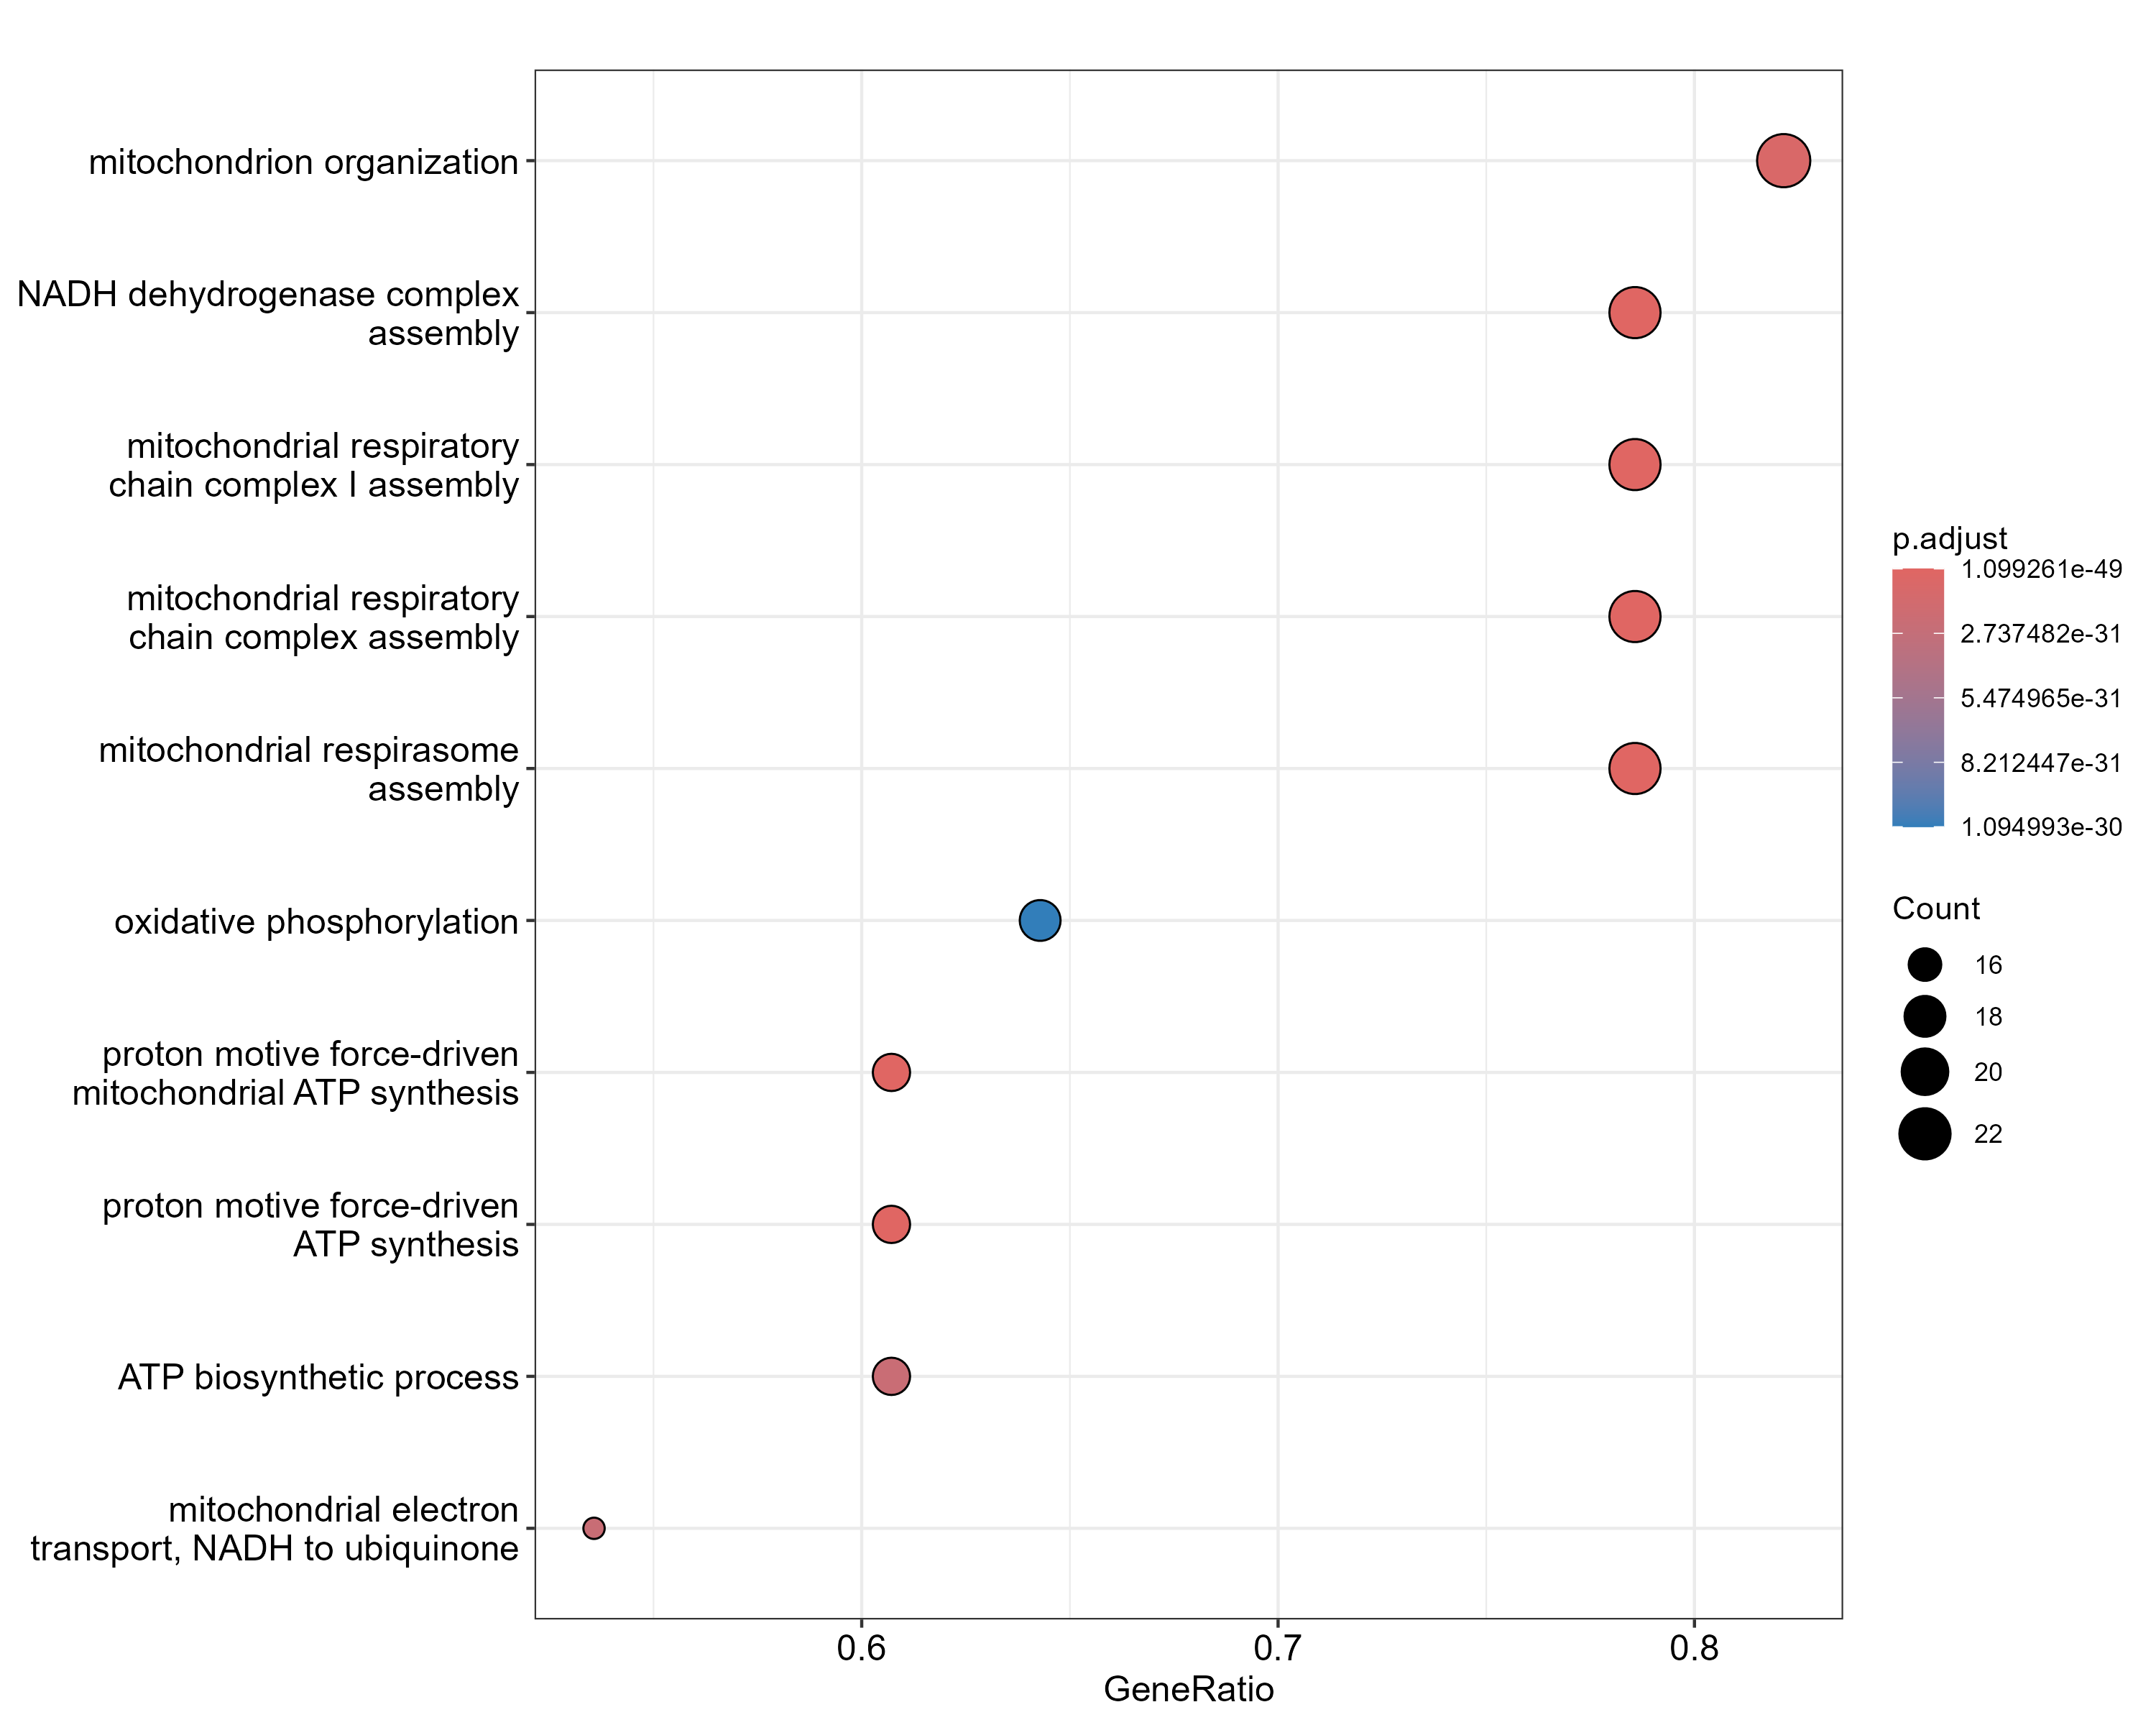
\includegraphics[width=0.8\textwidth]{figures/func_anal_res_genes_list.png}
	\caption{Análisis funcional de la lista de genes seleccionados}
	\label{fig:imagen3}
\end{figure}

\paragraph{}

El análisis funcional de los clústeres identificados por el algoritmo Fast Greedy confirma que los genes agrupados comparten funciones biológicas específicas relacionadas con la mitocondria, principalmente en la producción de energía y el ensamblaje de componentes mitocondriales. Los genes del primer y segundo clúster mostraron una conexión más estrecha, mientras que los del tercer clúster aparecen más segregados, con funciones posiblemente complementarias.

El análisis de los top nodes aporta una perspectiva adicional, destacando genes clave que actúan como nodos centrales en la red. Este enfoque combinado entre análisis funcional y estructural permite no solo entender las funciones principales de cada clúster, sino también identificar posibles reguladores centrales de la red de interacciones. Esto refuerza la utilidad de los análisis de clustering y funcionales como herramientas para explorar la complejidad biológica de los sistemas mitocondriales.
